%% ----------------------------------------------------------------
%% Thesis.tex -- MAIN FILE (the one that you compile with LaTeX)
%% ---------------------------------------------------------------- 

% Set up the document
\UseRawInputEncoding
\documentclass[a4paper, 12pt, oneside]{uet_thesis}
  % Use the "Thesis" style, based on the ECS Thesis style by Steve Gunn
\graphicspath{{Figures/}}  % Location of the graphics files (set up for graphics to be in PDF format)
%\renewcommand{\chaptername}{}
\usepackage{titlesec}
\usepackage{hyperref}
\titleformat{\chapter}[hang] 
{\normalfont\huge\bfseries}{\thechapter}{1em}{} 
% Include any extra LaTeX packages required
\usepackage[square, numbers, comma, sort&compress]{natbib}  % Use the "Natbib" style for the references in the Bibliography
\renewcommand{\cleardoublepage}{}
\usepackage{verbatim}  % Needed for the "comment" environment to make LaTeX comments

%\usepackage{vector}  % Allows "\bvec{}" and "\buvec{}" for "blackboard" style bold vectors in maths

\usepackage{url}
\usepackage{natbib}


\hypersetup{urlcolor=blue, colorlinks=true}  % Colours hyperlinks in blue, but this can be distracting if there are many links.

% remove the unnecessary spacing before and after the headings/subheadings

\titlespacing{\chapter}{0.1cm}{0.1cm}{0.1cm}
\titlespacing{\section}{0pt}{*1}{*1}
\titlespacing{\subsection}{0pt}{*0}{*0}
\titlespacing{\subsubsection}{0pt}{*0}{*0}

\setlength{\parskip}{6pt}
%\setlength{\parsep}{0pt}
%\setlength{\headsep}{0pt}
%\setlength{\topskip}{0pt}
\usepackage{atbegshi}% http://ctan.org/pkg/atbegshi
\AtBeginDocument{\AtBeginShipoutNext{\AtBeginShipoutDiscard}}

\begin{document}
\frontmatter
% Set up the Title Page
\title  {SmartGuide: A smart campus guide using BLE based indoor localization}
\session {2016 -- 2020}
\advisor {Dr. Sheikh Faisal Rasheed}
\authors {  % please enter the students names and registration numbers
\quad  2016-CE-72\\ \quad 2016-CE-54\\ \quad 2016-CS-159\\ \quad 2016-CE-81 }

\addresses  {\deptname \\ \univname}  % Do not change this here, instead these must be set in the "Thesis.cls" file, please look through it instead
\date       {\today}
\subject    {}
\keywords   {}

\clearpage\maketitle
\thispagestyle{empty}

%% ----------------------------------------------------------------

\clearpage  % Certification ended, now start a new page




%% ----------------------------------------------------------------
% End of the pre-able, contents and lists of things
% Begin the Dedication page
\setstretch{1.3}  % Return the line spacing back to 1.3
\pagestyle{empty}  % Page style needs to be empty for this page
%\dedicatory{For/Dedicated to/To my\ldots}


%% ----------------------------------------------------------------
%\pagestyle{fancy}  %The page style headers have been "empty" all this time, now use the "fancy" headers as defined before to bring them back

%% ----------------------------------------------------------------
%\lhead{\emph{Contents}}  % Set the left side page header to "Contents"
\tableofcontents  % Write out the Table of Contents
\newpage
%% ----------------------------------------------------------------
%\lhead{\emph{List of Figures}}  % Set the left side page header to "List if Figures"
\listoffigures  % Write out the List of Figures
\newpage
%% ----------------------------------------------------------------
%\lhead{\emph{List of Tables}}  % Set the left side page header to "List of Tables"
%\listoftables  % Write out the List of Tables

%% ----------------------------------------------------------------
\setstretch{1.5}  % Set the line spacing to 1.5, this makes the following tables easier to read
\clearpage  % Start a new page
%\lhead{\emph{Abbreviations}}  % Set the left side page header to "Abbreviations"
%\listofsymbols{ll}  % Include a list of Abbreviations (a table of two columns)
{
% \textbf{Acronym} & \textbf{W}hat (it) \textbf{S}tands \textbf{F}or \\
%\textbf{LAH} & \textbf{L}ist \textbf{A}bbreviations \textbf{H}ere \\
}

%% ----------------------------------------------------------------
% The Abstract Page

\clearpage  % Abstract ended, start a new page

%% ----------------------------------------------------------------
\mainmatter	  % Begin normal, numeric (1,2,3...) page numbering
%\pagestyle{fancy}  % Return the page headers back to the "fancy" style
\onehalfspacing
% Include the chapters of the thesis, as separate files
% Just uncomment the lines as you write the chapters

%\input{./Chapters/Chapter1} % Introduction 
%
%\input{./Chapters/Chapter2} % What to Write 

%\input{./Chapters/Chapter3} % Experimental Setup

%\input{./Chapters/Chapter4} % Experiment 1

%\input{./Chapters/Chapter5} % Experiment 2

%\input{./Chapters/Chapter6} % Results and Discussion

%\input{./Chapters/Chapter7} % Conclusion

%% ----------------------------------------------------------------
% Now begin the Appendices, including them as separate files

\addtocontents{toc}{\vspace{2em}} % Add a gap in the Contents, for aesthetics

%\appendix % Cue to tell LaTeX that the following 'chapters' are Appendices

%\input{./Chapters/AppendixA}	% Appendix Title

\newpage
\chapter{Introduction}
\section{Overview Of Project}
Advertising plays a critical role in marketing of a product. The ads released by the company represents the product and if not attractive enough or contain any factor disliked by the customer then its reputation can be damaged in an instant. Therefore, one needs to be careful about the customer’s likeness in order to avoid the financial and reputational damage. Every year, a company allocates a specific amount of marketing budget for the evaluation of advertisements realizing its importance in the promotion of a product. So, in order to provide a better and more reliable way to get customer’s feedback and to detect the effectiveness of an ad, an EEG based system for advertisement’s impact assessment will be established using machine learning techniques for automation of advertisement review analysis. In the proposed system, a low cost EEG headset i.e. Neurosky Mindwave Mobile will be used to collect the brain signals including different brain waves like alpha, beta, gamma and delta each of them being specific to a certain kind of activity of the subject viewing advertisements that aims in providing the statistics of the advertisement's impact and the likelihood of a person purchasing the advertised product. Different features like attention and meditation which are used to characterize the experience of the consumer will be extracted by continuously monitoring and analyzing the consumers’ brain activity. Then classification will be performed and results will be generated whether the customer liked or disliked the specific ad. This analysis will help us provide the statistical trend for a certain kind of advertisement on the basis of various factors. It will greatly help the marketing sector of multinational companies to improve their advertising campaign according to the feedback collected from different customers which will bring a revolutionary change in how they perceive their brand.
\section{Background}
Since the very beginning, marketers strive for understanding consumers preferences and what they were thinking in order to make their ads more productive by using traditional approaches. These techniques known as direct observation method include asking customers what they think and collecting data through surveys and focus groups and then its analysis, which require more manpower and has longer cycle in order to accomplish the results. Moreover, asking the person's review is unreliable because may be most of the time the person is not telling his/her genuine remarks. It is also more laborious, time consuming and less accurate. On the other hand, advertisements are considered very important nowadays as a huge amount of money is being spent on them globally. If we take a look at its global statistics, the latest Dentsu Aegis Network Ad Spend forecasts show in 2019 the growth will increase by 3.8\%, amounting to US\$625 billion \cite{b1}. If we look back in year 2016, the advertising global spending was worth \$500billion\cite{b2}.And if marketing expense i.e. research, marketing,etc.then the total worth of industry
becomes \$965 billion. Global advertising spending from 2010 to 2018 (in billion U.S.dollars) is shown in Figure 1 \cite{b3} below:

\begin{figure}[htbp]
\centerline{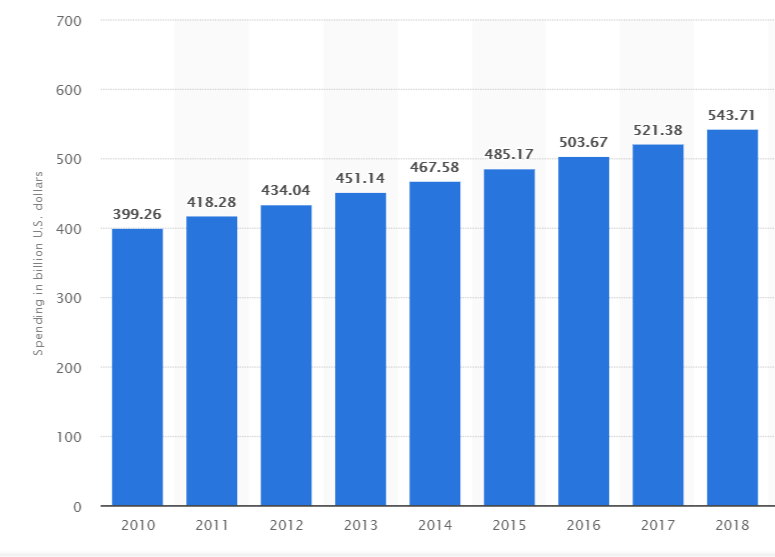
\includegraphics[scale=0.6]{Figure1.png}}
\caption{Global advertising spending from 2010 to 2019 (in billion U.S. dollars)}
\label{Figure 1}
\end{figure}
Therefore, considering the importance of ads, one cannot rely on such traditional techniques and need some advancement.\par
Some current assessment methods also contains indirect inference from observing changes in customer’s behavior after releasing the advertisement which requires a lot of time and also ad campaign has to be launched beforehand which most probably means cost is already at risk. Similarly some techniques like interpreting person's facial expression and inspecting thoroughly their hand–eye coordination are also applied. All these methods have some drawbacks like some are time consuming while other are ambiguous and may lead one to take inappropriate actions to reach the goal. Whereas, directly collecting the EEG brain waves in order to get the customer’s feedback will be less time consuming and will yield more accurate result.

\section{Motivation}
In today’s world, advertising is a huge business. It gives important information in productive and cost-effective way regarding the services and products and is a powerful tool of competition. Therefore, advertising helps the economy to function smoothly by facilitating the entry of advanced and unfamiliar products and new brands into the market. As we already know that consumer’s opinion plays a major role in making an advertisement . Keeping that in mind, Some major aspects that motivated us to opt this project are:

\begin{itemize}
\item The advertising industry in Pakistan is growing anually at a rate of 10-12pc and it worth \$650 million because of continuously emerging urban middle class and increase in consumerism, purchasing power, and an expanding economy \cite{b2}. So, we need some reliable methods to make our advertisements better and avoid the financial risk. 
\item In Pakistan, advertising sector is frequently criticized because of its lack of creativity and detest of the consumers. The need of the hour is to create productive ads according to customer’s likeness as consumer confidence matters the most \cite{b4}.
\item Nowadays, advertising campaigns are represented by creative and productive and ideas rather than expensive brand endorsements. What matters is the material that clicks in customer's minds. Current campaign shows that communications is the important part and gone are the days when you could just make consumer accept an idea by continuously showing it. 
\item Currently, Pakistan is a hot  market for multinationals as it is growing very rapidly and that is why they are increasing the spend on advertsement. TV remains the biggest medium for media spend in Pakistan with Rs30 billion spending. As the country is spending so much in advertising, the ads must be according to consumer’s likeness to reduce the risk of loss.
\end{itemize}
\newpage
\chapter{Objectives}
The use of brain signals to study one’s response is a very effective way for analysis. It gives a proper insight to what is one’s behavior and what decision one will make regarding something. 

\section{Industry Objectives}
The success of any product highly depends on its marketing and advertisement analysis is very important in brand marketing. Every year companies set a specific marketing budget for their advertising campaign. People are asked to fill questionnaires in order to record their response regarding their brand or a particular advertisement for their brand. However, such responses are mostly ambiguous, biased and does not help in a fruitful assessment. To overcome this problem, our aim is to use the technique of neuro-marketing and automate the consumer feedback mechanism for analysis of any kind\cite{b6}. It is supposed to guide the marketers to the right product designs and ad messages to boost sales. Many companies like Hyundai, Google, Walt Disney, Microsoft, Chevron etc\cite{b5}. Few of the industrial objectives are as follows:

\begin{itemize}
\item The system must allow the analysts to fill in the gaps left by traditional marketing methods.
\item It must help the marketing analysts understand the consumer preferences in order to improve brand quality, advertisements, packaging etc.
\item Our project should focus on the study of brain responses to marketing stimuli which will revolutionize marketing sector of industries.
\item It must be so economical causing the industries to save on their marketing expenses by recording consumers’ response in an effective and efficient way\cite{b7}.
\item System must cut off losses of industries in marketing sector, by making them predict consumers’ response using advanced techniques accurately.
\item Main aim of our project is to develop a system that is cost effective and error free than the previously designed systems which will eventually lead the industrial field to progress\cite{b8}.
\item It must help the industrial sector to make necessary changes wherever required in the product or advertisement beforehand by analyzing consumers’ behavior.
\end{itemize}

\section{Research Objectives}
These objectives involve, a comprehensive study of all the research done in the system’s development field and then on its basis, developing a system that can be able to acquire brain signals and classify them in order to predict the results accurately and in turn should be better than the previously designed systems\cite{b9}. Few of the research objectives are as follows:

\begin{itemize}
\item The main objective is to acquire the brain signals in a csv file from the headset to have a closer look at the signals attained and to understand them better.
\item Project’s research is based on correct distinction between different brain signals, representing different emotions and behavior. So initially the research is based on the understanding different signals connected with different emotions. In order to draw conclusions better.
\item The toughest part is the detection and classification of brain signals into different emotions using different classifiers, whichever is more accurate in prediction\cite{b10}.
\item There should be a thorough research, so that the developers must be able to discover new techniques which are more efficient and faster than previous ones.
\item Techniques that are not yet used must be preferre\cite{b20}. Such techniques must be understood properly and used in such a way that they help in the development of an efficient and intelligent system that is able to analyze human emotions more accurately than older systems.
\end{itemize}

\section{Academic Objectives}
Such objectives play a basic role in developers’ career as the goal of this project work is to gain and enhance skills of development and have a deeper insight of this field. 
Few of the academic objectives are as follows:

\begin{itemize}
\item The main goal of this project is to allow the developers learn major areas of computer field more specifically machine learning and signal processing.
\item Developers must learn problem solving techniques in order to solve real world problems that they encounter in their career.
\item The developers should be exposed to new technologies which help them connect with the technological world in a better way.
\item The developers must implement the test and trial method. They must test different techniques and use those that are more suitable for the project. This will also help them in their future works.
\item Practical performance must be worked upon more and more.
\item The developers must practice risk and change management in the course of their project development. Also, they would be able to polish their decisive power.
\item Developers must learn to meet the deadlines. This will teach them professionalism, which will help them in their future jobs.
\item The developers must work as a team and learn to compromise in different situations. They must also learn to work under or as a team lead. This will help them in broadening their vision.
\item They should be able to understand the importance of commitment and should stay committed to their work.
\end{itemize}
\newpage
\chapter{Goal of the project}
\newpage
\chapter{Scope of the project}
The project involves automation of advertisement review analysis.There will be an app for Android based systems. After establishing connectivity,the user will be shown an advertisement of one of the four categories, during which  brain signals of the subject will also be recorded using the Neurosky Mobile 2 headset. EEG data will be stored in a csv file that is specific to each subject. After showing each add, we will ask the subjects to fill in the questioannaires in order to determine subject's response to the ad so to get labeled data. We will then use this labeled and unlabled data to train our model. This will then be classified into two classes, in order to predict whether the ad is likeable or  not. However, we are also determined to achieve the extent to which the subject liked the ad or to which extent one disliked it. The app will not only display per subject values of different levels of emotions but it will also show wehether it is likeable by the person or not.
\newpage
\chapter{Target Audience}
\section{Marketers and Consumer}
Prposed system can be helpful for the company employees who work as marketers in a company in B2B(Bussiness to Bussines) and B2C(Bussiness to Consumer) environments \cite{b21}. In B2B context the marketers are trying to convince a single person and in B2C they want to convince the decision maker in a company. They used the system to adopt persuasive strategy from knowing what is triggering the feeling of satisfaction in the brain shown by application and try to convince them with the proof to buy the product or signing a partnership deal[22] .   

\section{Educational Admministrators}

Administrators in the educational system can used our system to analyze important features related to the learning performance of the student while they are watching educational videos and use it as factors in the adjustment of instructional methods \cite{b23}. That leads to become a better institution and enhance the learning capability of students. 

\section{Researchers}
Researchers can used our system to know the reaction of individuals to make progress in their research in neuromarketing.

\section{General Public}
Fresher in entertainment industry or any person who wants to know the honest reaction of people on their personal created video can use our application. Accordingly make changes and make their work better and this will decrease the chance of failure. 

\newpage
\chapter{Possible applications of work}

\section{Marketing sector}
The proposed system will help the companies to improve their promotional advertisement video and to make it more attractive and productive by giving them response of different customer’s. Therefore, it will eventually upgrade their marketing. 
\section{Advertising industry}
As it is the global industry of public relations and marketing companies, when the proposed system will enhance the advertisements to provide effective information about products and services in an efficient manner, it will be beneficial for the advertising industry as well.
\section{Increase in economy}
In a country where consumer spending determines the long run of the economy advertising motivates them to pay more. So, by playing a positive role in both marketing sector and advertising industry , which provides goods, services and jobs, proposed system will deep down increase the economy of the country.
\section{Entertainment industry}
As the system gives the feedback on a video, it can be used in entertainment industry as well to enhance the music video’s, short movies, different parts of movies or dramas etc. according to the viewer’s taste before releasing them.  
\section{Education sector}
By getting the student’s feedback on online lectures, proposed system can be used to upgrade the teaching methods accordingly. 
\section{Research in Neuromarketing}
In the proposed system, neuromarketing (the use of modern brain science to measure the impact of marketing and advertising on consumers) will be used. So, a person doing research in this field can use the system.
\section{Other}
With some advancements if the proposed system is trained to work without the video then it can be used in the classrooms to get the student’s feedback about teachers or the classroom environment to improve education system and also to enhance a company’s environment by getting employee’s feedback etc. 

\newpage
\chapter{Existing Systems}
\section{Comparison of Existing Systems}
In recent years, indoor localization systems have been great significant research activity and of growing interest for their great expected social impact. In spite of the numerous research advances, no canned solutions have yet been defined. The diversity and heterogeneity of applications, scenarios, sensor and user requirements, make it difficult to create uniform solutions. There are multiple solutions present in research area for indoor localization. Here are the comparisons of few of them: 

\begin{figure}[htbp]
\centerline{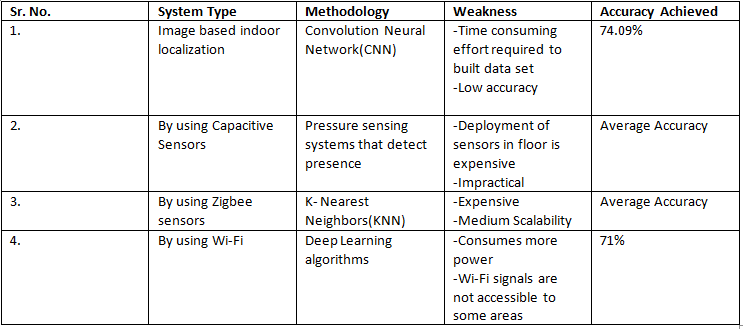
\includegraphics[scale=0.7]{abc.png}}
\caption{Comparison of existing systems}
\label{Table3}
\end{figure}

\section{Drawbacks of Existing Systems}
There are many drawbacks in existing systems. In some systems, camera is required for indoor positioning which is obtrusive for some users. High cost and effort is required for the deployment of indoor localization infrastructure. Most of the existing systems have medium or low accuracy. In image based indoor localization, time consuming effort is required for built data sets. Wi-Fi fingerprinting is relatively better than other systems because of finding position by using already deployed infrastructure. But its main drawback is that it consumes more power. There are some spots where Wi-Fi access points would be difficult to power. There are some areas where Wi-Fi signals are not accessible. In our proposed system, we will find indoor location using BLE beacons. BLE beacons are small in size, light weight and cheaper then Wi-Fi. BLE consumes less power than Wi-Fi. BLE beacons are usually battery powered, which are more flexible and easier deployed than sensors used by existing systems. BLE RSS signals can have a higher sample rate than Wi-Fi RSS signals (0.25 Hz~2 Hz). Our proposed system will provide more accuracy than existing systems and also it is unobtrusive. So, our proposed system will overcome the shortcomings in existing systems. Furthermore, our system will not only predict location but also provide information of that location and nearby location in text, videos, audio and images form which is missing in existing systems because they find indoor positioning for different purposes.




\newpage
\chapter{Problem Statement}
We will be developing a fast, accurate and efficient system to get a person’s feedback and state of brain properly in order to understand what customers are thinking to prevent any negative impact from our advertisement and changing the policies accordingly. 

\newpage
\chapter{Proposed System}
Proposed system consists of four modules:

\section{Headset Connectivity}
User needs to properly wear the headset by placing the single electrode on the frontal lobe and placing the reference electrode on ear lobe and connect it with the system using Bluetooth and ThinkGear Connector.
\section{Data Acquisition}
Brain signals will be acquired in a csv file while the user is watching the advertisement to collect direct response.
\section{Response on advertisement}
As soon as the advertisement finishes the user can view the real response on the advertisement in the form of weather the particular person liked it or not.
\section{Overall Response}
All the individual responses will be collected of a particular advertisement to let the company know whether people liked it or not.
\section{Existing system flow chart}
The flow charts of existing systems are shown in Figures 3, 4 and 5. These are the methodologies of some extising systems which were better than others. We will be using these researches in order to derive our own methodology.
\begin{figure}[htbp]
\centerline{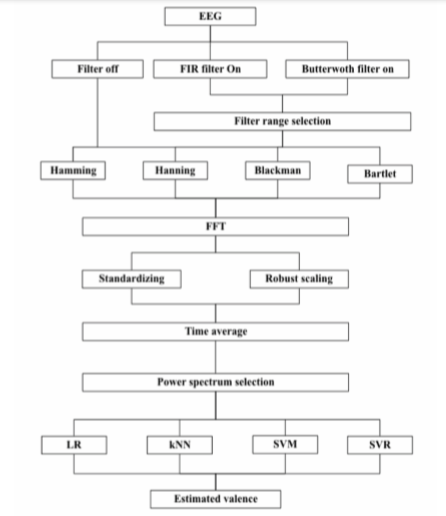
\includegraphics[scale=0.8]{Existing1.png}}
\caption{Flowchart of Existing system  \cite{b1}}
\label{Table4}
\end{figure}

\begin{figure}[htbp]
\centerline{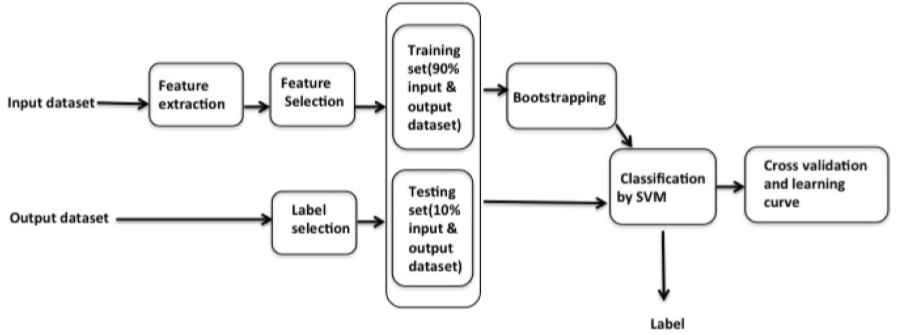
\includegraphics[scale=0.7]{Existing2.png}}
\caption{Flowchart of Existing system  \cite{b15} }
\label{Table4}
\end{figure}
\newpage
\begin{figure}[htbp]
\centerline{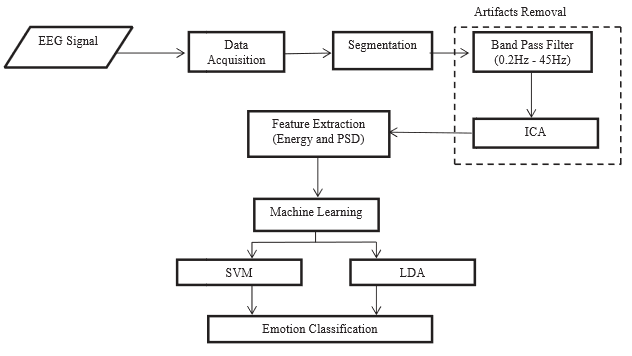
\includegraphics[scale=0.8]{Existing3.png}}
\caption{Flowchart of Existing system  \cite{b18}}
\label{Table4}
\end{figure}



\newpage
\chapter{Feasibility Study}
\section{Technical Feasibility}

For the development of proposed system, we will use latest technologies. Android studio is used for development of android application. Weka API is used for machine learning. Weka is a machine learning library for Java. BLE beacons are used for capturing RSSI signals. BLE beacons are small in size, light weight, cheaper and easily available. Android application connects with BLE beacons through Bluetooth. BLE RSS signals can have a higher sample rate than Wi-Fi RSS signals (0.25 Hz 2 Hz). BLE beacons can easily deploy as compared to other sensors existing in market. We have necessary skill sets for the implementation of this project. This project requires understanding of machine learning, development of android application and understanding of how application communicate with BLE beacons and server. We are all familiar with machine learning and recently we are trying to learn Android Application development. Our supervisor and co-advisor are very supportive and they have all necessary skill sets to properly guide us. So, considering all these things, it is clear that our project is highly technical feasible and higher chances of completion.

\section{Operational Feasibility}
Operational feasibility means whether a proposed system is to be feasible at operational level. Our proposed system is basically a guided tool that not only tells room level predication but also information related to that room and nearby rooms. This project will guide person who is not much familiar with visiting place. In our case, visiting place will be university campus. Students who do not familiar with campus rooms and activities are much likely to use this application. For this purpose, we conduct a market survey

\section{Economical Feasibility}
Economical feasibility means whether a project is economically feasible by analyzing the cost required for developing and using this project. For deploying an android application on play store requires 25 dollars which is nearly equal to Rs 3,921.25 

\newpage
\chapter{System Requirements}

\section{Hardware Requirement}

\begin{itemize}
\item Neurosky MindWave Mobile 2
\item Android Phone: Android 4 or later
\item PC with window 7/8/8.1/10[30].
\begin{itemize}
     \item Processor: Intel Core Duo or equivalent
     \item Memory: 1GB or more
     \item Video: DirectX 9.0 or greater
     \item Hard disk: 2.5GB free disk space
     \item Wireless: Bluetooth
\end{itemize}
\end{itemize}

\section{Software Requirement}
\begin{itemize}
\item Unity (work with C\#, android platform)
\item Python (3.6 or older versions)
\item Bluetooth
\item ThinkGear Connector
\item Framework for connecting unity and python
\item Python web framework Django
\end{itemize}


\newpage
\chapter{SWOT Analysis}

During the life cycle of a research based project, there are many hindrances and challenges one faces and it is important to keep note of such limitations and problems beforehand. So that necessary steps can be taken.

\section{Headset Connectivity}
As the headset is a very sensitive device, so one of the challenges is the connectivity of the headset which can be affected by electrical interferences and weak batteries as shown in the Fig. 4\cite{b31}.

\begin{figure}[htbp]
\centerline{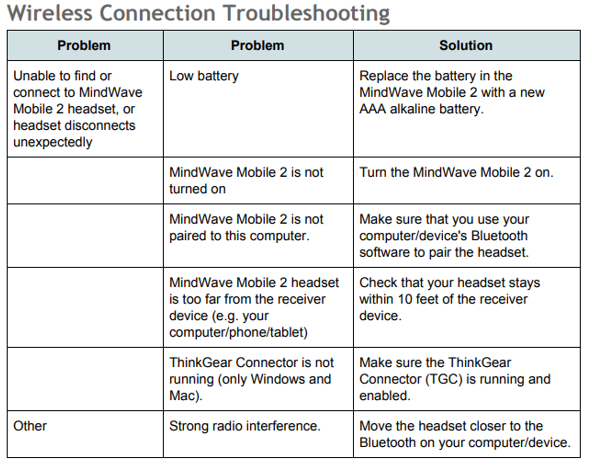
\includegraphics[scale=0.7]{Table1.png}}
\caption{Wireless Connection Troubleshooting}
\label{Table1}
\end{figure}

\section{Dataset Collection}
The dataset collection of the brain signals while the subject is watching the advertisement is the main challenge.

\section{Brain signal Variations}
Brain signals vary from person to person. So, in order to have accurate results more training samples are needed in order to get reliable insights from the studies. Greater samples require greater time\cite{b32}.

\begin{figure}[htbp]
\centerline{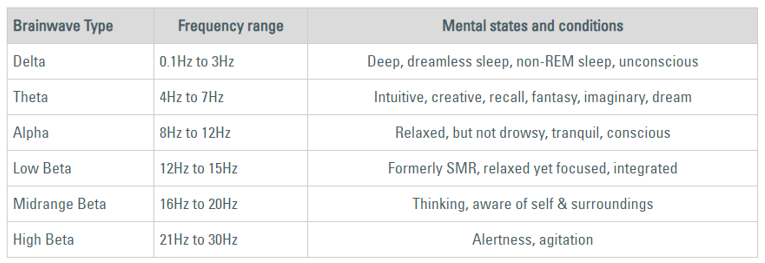
\includegraphics[scale=0.7]{Table2.png}}
\caption{Signals and Emotions}
\label{Table2}
\end{figure}

\section{Limited Signal Range}

The work is performed on limited brain signals provided by the EEG headset that are responsible for various emotions. So, the system will be able to perform on only those signals and will give analysis within those boundaries. As shown Fig. 5

\section{Environmental Setup}
Reactions observed in a lab test environment may be somewhat different from the actual buying environment which may affect the results. In other word, it may challenge the validity of the assessment results.






%\input{./Chapters/AppendixB} % Appendix Title

%\input{./Chapters/AppendixC} % Appendix Title

\addtocontents{toc}{\vspace{2em}}  % Add a gap in the Contents, for aesthetics
\backmatter

%% ----------------------------------------------------------------
\newpage
\chapter{Refrences}
\begin{thebibliography}{00}
\bibitem{b1} Global Ad Spend Forecasts. [online] Available at: https://assets-eu-01.kc-usercontent.com/6d786bf2-d07c-0171-96cf-6e7595ee7cc6/678c6758-c5a7-498e-b718-ea3d3cbeafbb/
\bibitem{b2} PakistanToday(2017). The world of advertising – An overview. [online]  Available at: https://www.pakistantoday.com.pk/2017/05/28/the-world-of-advertising-an-overview/
\bibitem{b3} Statista. Global advertising spending from 2010 to 2019 (in billion U.S. dollars). [online]  Available at: https://www.statista.com/statistics/236943/global-advertising-spending/
\bibitem{b4} Pas. THE EVER EVOLVING ADVERTISING INDUSTRY OF PAKISTAN – IT’S TIME TO TAKE CHANCES. [online] Available at: https://pas.org.pk/the-ever-evolving-advertising-industry-of-pakistan-its-time-to-take-chances/

\bibitem{b5}Forbes (2019). Neuro-marketing: Companies Use Neuroscience for Consumer Insights. [online] Available: https://www.forbes.com/forbes/2009/1116/
\bibitem{b6} Nero-marketing by Roger Dooley: What is neuro-marketing? [online] Available: https://www.neurosciencemarketing.com/blog/articles/what-is-neuromarketing.htm
\bibitem{b7} Luis Miguel Soria Morillo, Juan Antonio Alvarez Garc´ıa, Luis Gonzalez-Abril, and J.A. Ortega Ramirez - Advertising Liking Recognition Technique Applied to Neuromarketing by Using Low-Cost EEG Headset - Conference Paper: April 2015. [online] Available: https://www.researchgate.net/publication/300901819
\bibitem{b8} Eminent SEO (2017).  What Is Neuro-marketing and Is It Better Than Traditional Marketing? [online] Available: https://www.eminentseo.com/blog/what-is-neuromarketing-vs-traditional-marketing/
\bibitem{b9}The Open University [GB] Project Research Objectives. [online] Available: https://www.open.edu/openlearncreate/mod/oucontent
\bibitem{b10}Aayush Bhardwaj, Ankit Gupta, Pallav Jain, Asha Rani, Jyoti Yadav - Classification of human emotions from EEG signals using SVM and LDA Classifiers  -  2015 2nd International Conference on Signal Processing and Integrated Networks (SPIN). [online] Available: https://ieeexplore.ieee.org/document/7095376

\bibitem{b11}Ogino, M. and Y. Mitsukura. A Mobile Application for Estimating Emotional Valence Using a Single-Channel EEG Device. in 2018 57th Annual Conference of the Society of Instrument and Control Engineers of Japan (SICE). 2018.
\bibitem{b12}Morillo, L.M.S., et al. Advertising liking recognition technique applied to neuromarketing by using low-cost EEG headset. in International Conference on Bioinformatics and Biomedical Engineering. 2015. Springer.
\bibitem{b13}Oon, H.N., A. Saidatul, and Z. Ibrahim. Analysis on Non-Linear Features of Electroencephalogram (EEG) Signal for Neuromarketing Application. in 2018 International Conference on Computational Approach in Smart Systems Design and Applications (ICASSDA). 2018.
\bibitem{b14}Soria Morillo, L.M., et al., Discrete classification technique applied to TV advertisements liking recognition system based on low-cost EEG headsets. BioMedical Engineering OnLine, 2016. 15(1): p. 75.
\bibitem{b15}Wei, Z., et al., Using Support Vector Machine on EEG for Advertisement Impact Assessment. Frontiers in Neuroscience, 2018. 12(76).
\bibitem{b16}Terasawa, N., et al. Tracking liking state in brain activity while watching multiple movies. in Proceedings of the 19th ACM International Conference on Multimodal Interaction. 2017. ACM.
\bibitem{b17}Ang, H.J.Y., G.A. Sanchez, and J.A. Pascual, Detecting interest in video advertisements using EEG data analysis. Philippine Information Technology Journal, 2016. 7(1): p. 4-12.
\bibitem{b18}Bhardwaj, A., et al. Classification of human emotions from EEG signals using SVM and LDA Classifiers. in 2015 2nd International Conference on Signal Processing and Integrated Networks (SPIN). 2015.
\bibitem{b19}Yadava, M., et al., Analysis of EEG signals and its application to neuromarketing. Multimedia Tools and Applications, 2017. 76(18): p. 19087-19111.


\bibitem{b20}Zhen Wei, Chao Wu1, Xiaoyi Wang, Akara Supratak, Pan Wang1 and Yike Guo – Using Support Vector Machine on EEG for Advertisement Impact Assessment – US National Library of Medicine National Institutes of Health: Frontiers of Neuro-Science March 2018  Available: https://www.ncbi.nlm.nih.gov/pubmed/29593481


\bibitem{b21}C\&EN Media Group(July 02, 2018). Your Neuromarketing Guide, Step 1: Defining Your Unique Target Audience   [online] Available:https://acsmediakit.org/blog/neuromarketing-step-1-defining-your-unique-target-audience/
\bibitem{b22} Productivity Revolution. How modern B2B marketers can benefit from Neuromarketing .[online] Available: https: //blog.alore.io/neuromarketing-in-b2b-marketing/
\bibitem{b23} ieeexplore.ieee.org(2017) .  Adaptive learning system for E-learning based on EEG brain signals.  [online] Available:https://ieeexplore.ieee.org/document/8229382l

\bibitem{b24} Brainwave Sensing Headset.[online] Available: https://store.neurosky.com/pages/mindwave
\bibitem{b25} Using Support Vector Machine on EEG for Advertisement Impact Assessment Zhen Wei1*, Chao Wu1,2, Xiaoyi Wang3, Akara Supratak1, Pan Wang1 and Yike Guo1*.[online] Available: https://www.frontiersin.org/articles/10.3389/fnins.2018.00076/full
\bibitem{b26} BBC News. From Pepsi to Nivea: Some of the worst advertising fails By Leisha Chi BBC Business reporter 6 April 2017.[online] Available: http://bbc.com/news/business-39511906
\bibitem{b27} The Disadvantages of Bad Publicity by Marie Beauchamp; Updated July 24, 2019.[online] Available: https://yourbusiness.azcentral.com/disadvantages-bad-publicity-3495.html
\bibitem{b28} LAB TALK (2017). R\&D with Commercially Available EEG Headsets . [online] Available: https://sapienlabs.org/rd-commercially-available-eeg-headsets/
\bibitem{b29} NeurotechEDU – Educational Materials for Neurotechnology. COMPARE AND CONTRAST Available: Consumer EEG Headsets. [online] Available: http://learn.neurotechedu.com/headsets/
\bibitem{30} MindWave Mobile 2: User GuideMay 14, 2018. [online] Available: http://download.neurosky.com/public/Products/

\bibitem{b31}Mindwave Mobbile 2: User Guide [online] Available: http://download.neurosky.com/public/Products/
\bibitem{b32}NeuroSky – MindSet. [online] Available: http://developer.neurosky.com/docs/



\end{thebibliography}


%\label{References}
%\lhead{\emph{References}}  % Change the left side page header to "References"
%
%\bibliographystyle{plainnat}  % Use "unsrtnat" BibTeX style for formatting the references
%%
%\bibliography{references}  % The references information are stored in the file named "references.bib"

\end{document}  % The End
%% ----------------------------------------------------------------
